\documentclass[10pt,a4paper]{scrartcl}
\usepackage[utf8]{inputenc}
\usepackage{amsmath}
\usepackage{amsfonts}
\usepackage{amssymb}
\usepackage{graphicx}

\usepackage[bottom = 1in, left = 0.5in, right = 0.5in, top = 1in]{geometry}

\usepackage[english]{babel}
\usepackage[autostyle]{csquotes}
\usepackage{mathptmx}

\usepackage[labelfont=bf]{caption}

\usepackage[default, scale=0.95]{opensans}

\usepackage[T1]{fontenc}

\usepackage{fixltx2e}

\title{My neat title here}
\subtitle{Figures}
\date{}

\begin{document}
\maketitle

\begin{figure}[h]
	\centering
	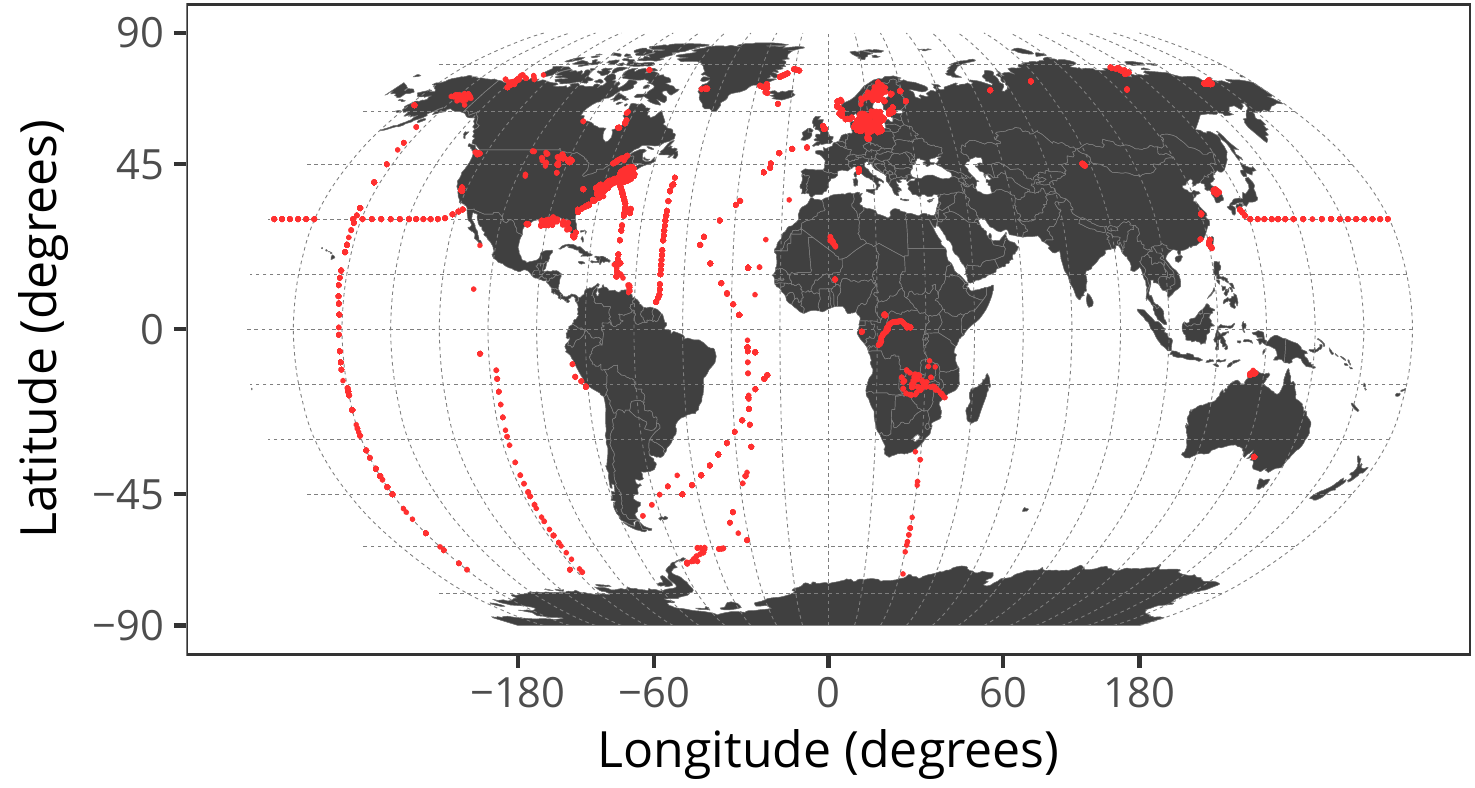
\includegraphics[scale = 1]{../../graphs/fig1}
	\caption{World map showing the spatial distribution of the observations extracted from the literature ($n = xxx$).}
\end{figure}

\clearpage
\newpage

\begin{figure}[h]
	\centering
	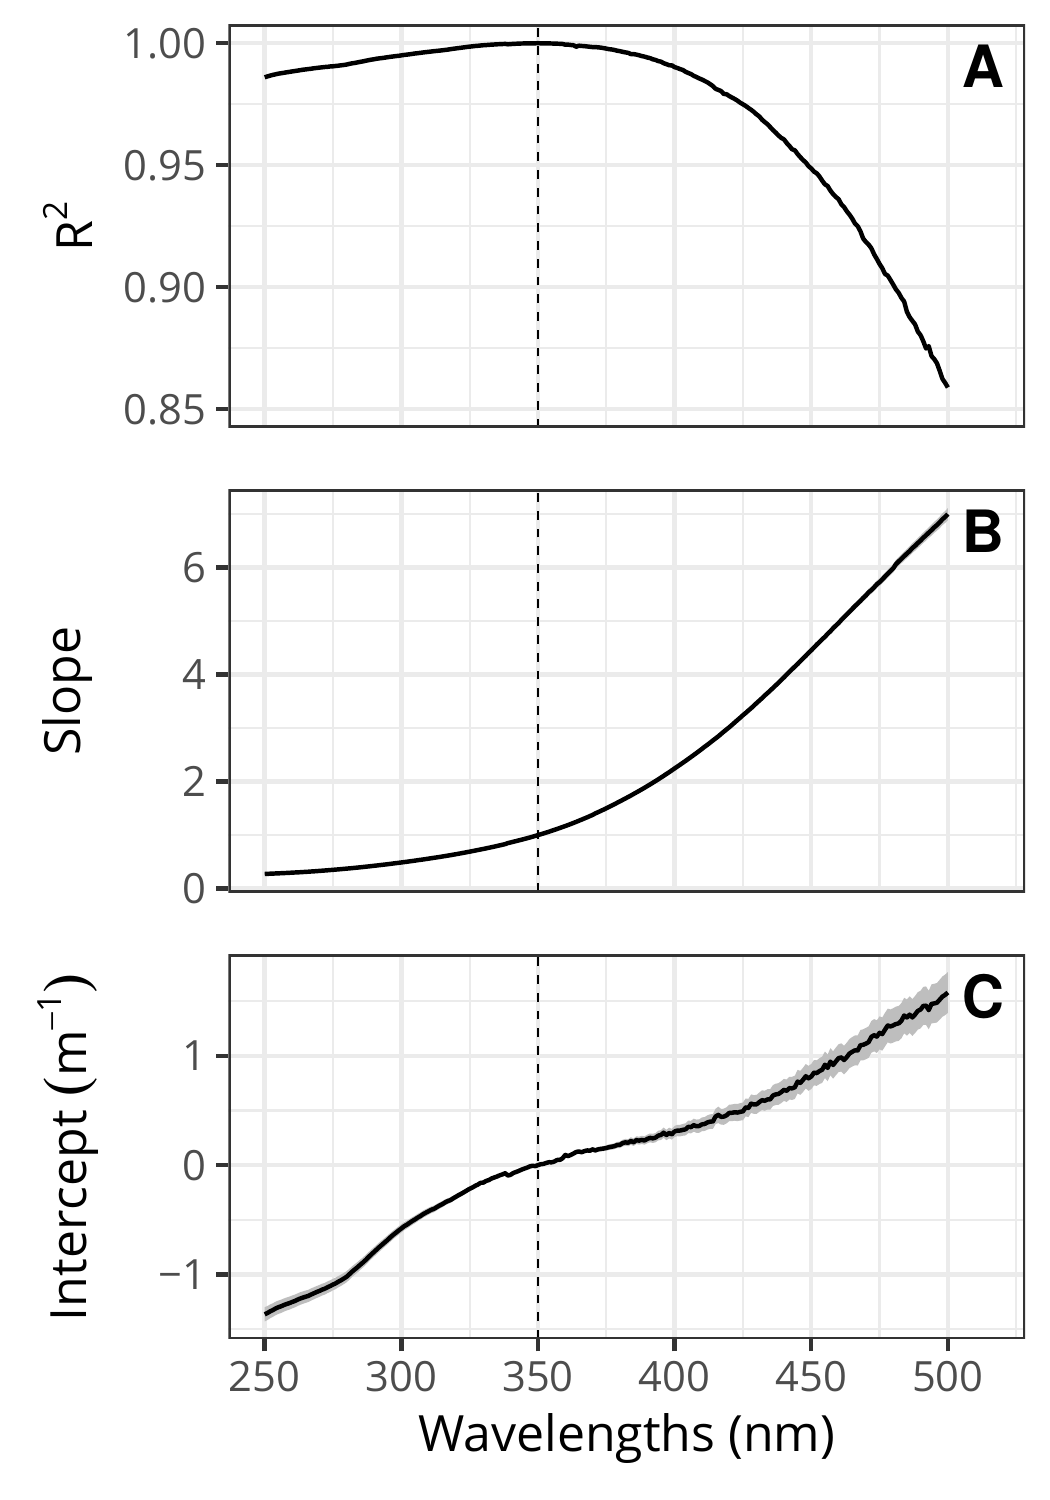
\includegraphics[scale = 1]{../../graphs/fig2}
	\caption{Results of the linear regressions between a\textsubscript{CDOM}(350) and a\textsubscript{CDOM}($\lambda$). (\textbf{A}) Determination coefficients ($R^2$), (\textbf{B}) slopes and (\textbf{C}) intercepts of the linear regressions. Panels contain the results of 251 linear models, each based on 2321 data points. Note that at $\lambda = 350$ nm, $R^2 = 1$, slope = 1 and intercept = 0.}
\end{figure}

\clearpage
\newpage

\begin{figure}[h]
	\centering
	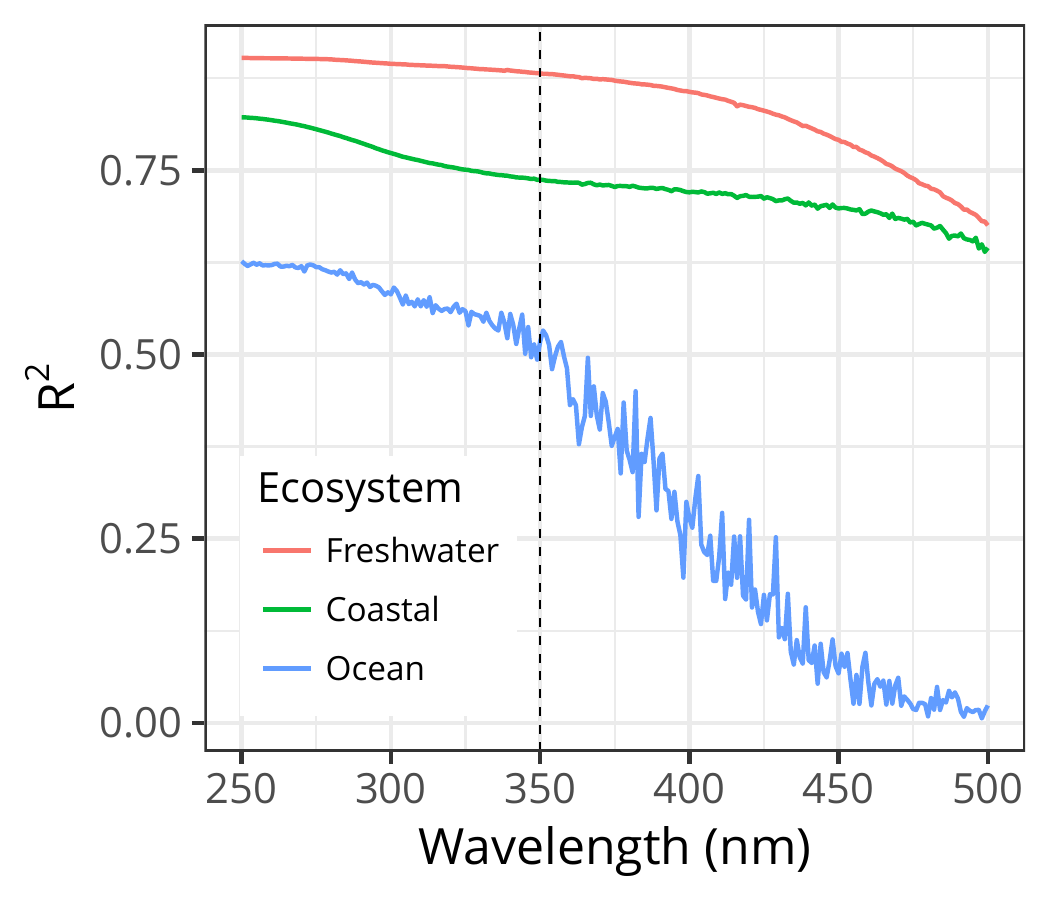
\includegraphics[scale = 0.75]{../../graphs/fig3}
	\caption{Boxplots showing the distribution of (\textbf{A}) absorption coefficients at 350 nm ($a_{CDOM}(350)$), (\textbf{B}) dissolved organic carbon (DOC) and (\textbf{C}) the \textit{so-called} $a^*$. Y-axis are log-transformed given the wide ranges spanned by the data.}
\end{figure}

\clearpage
\newpage

\begin{figure}[h]
	\centering
	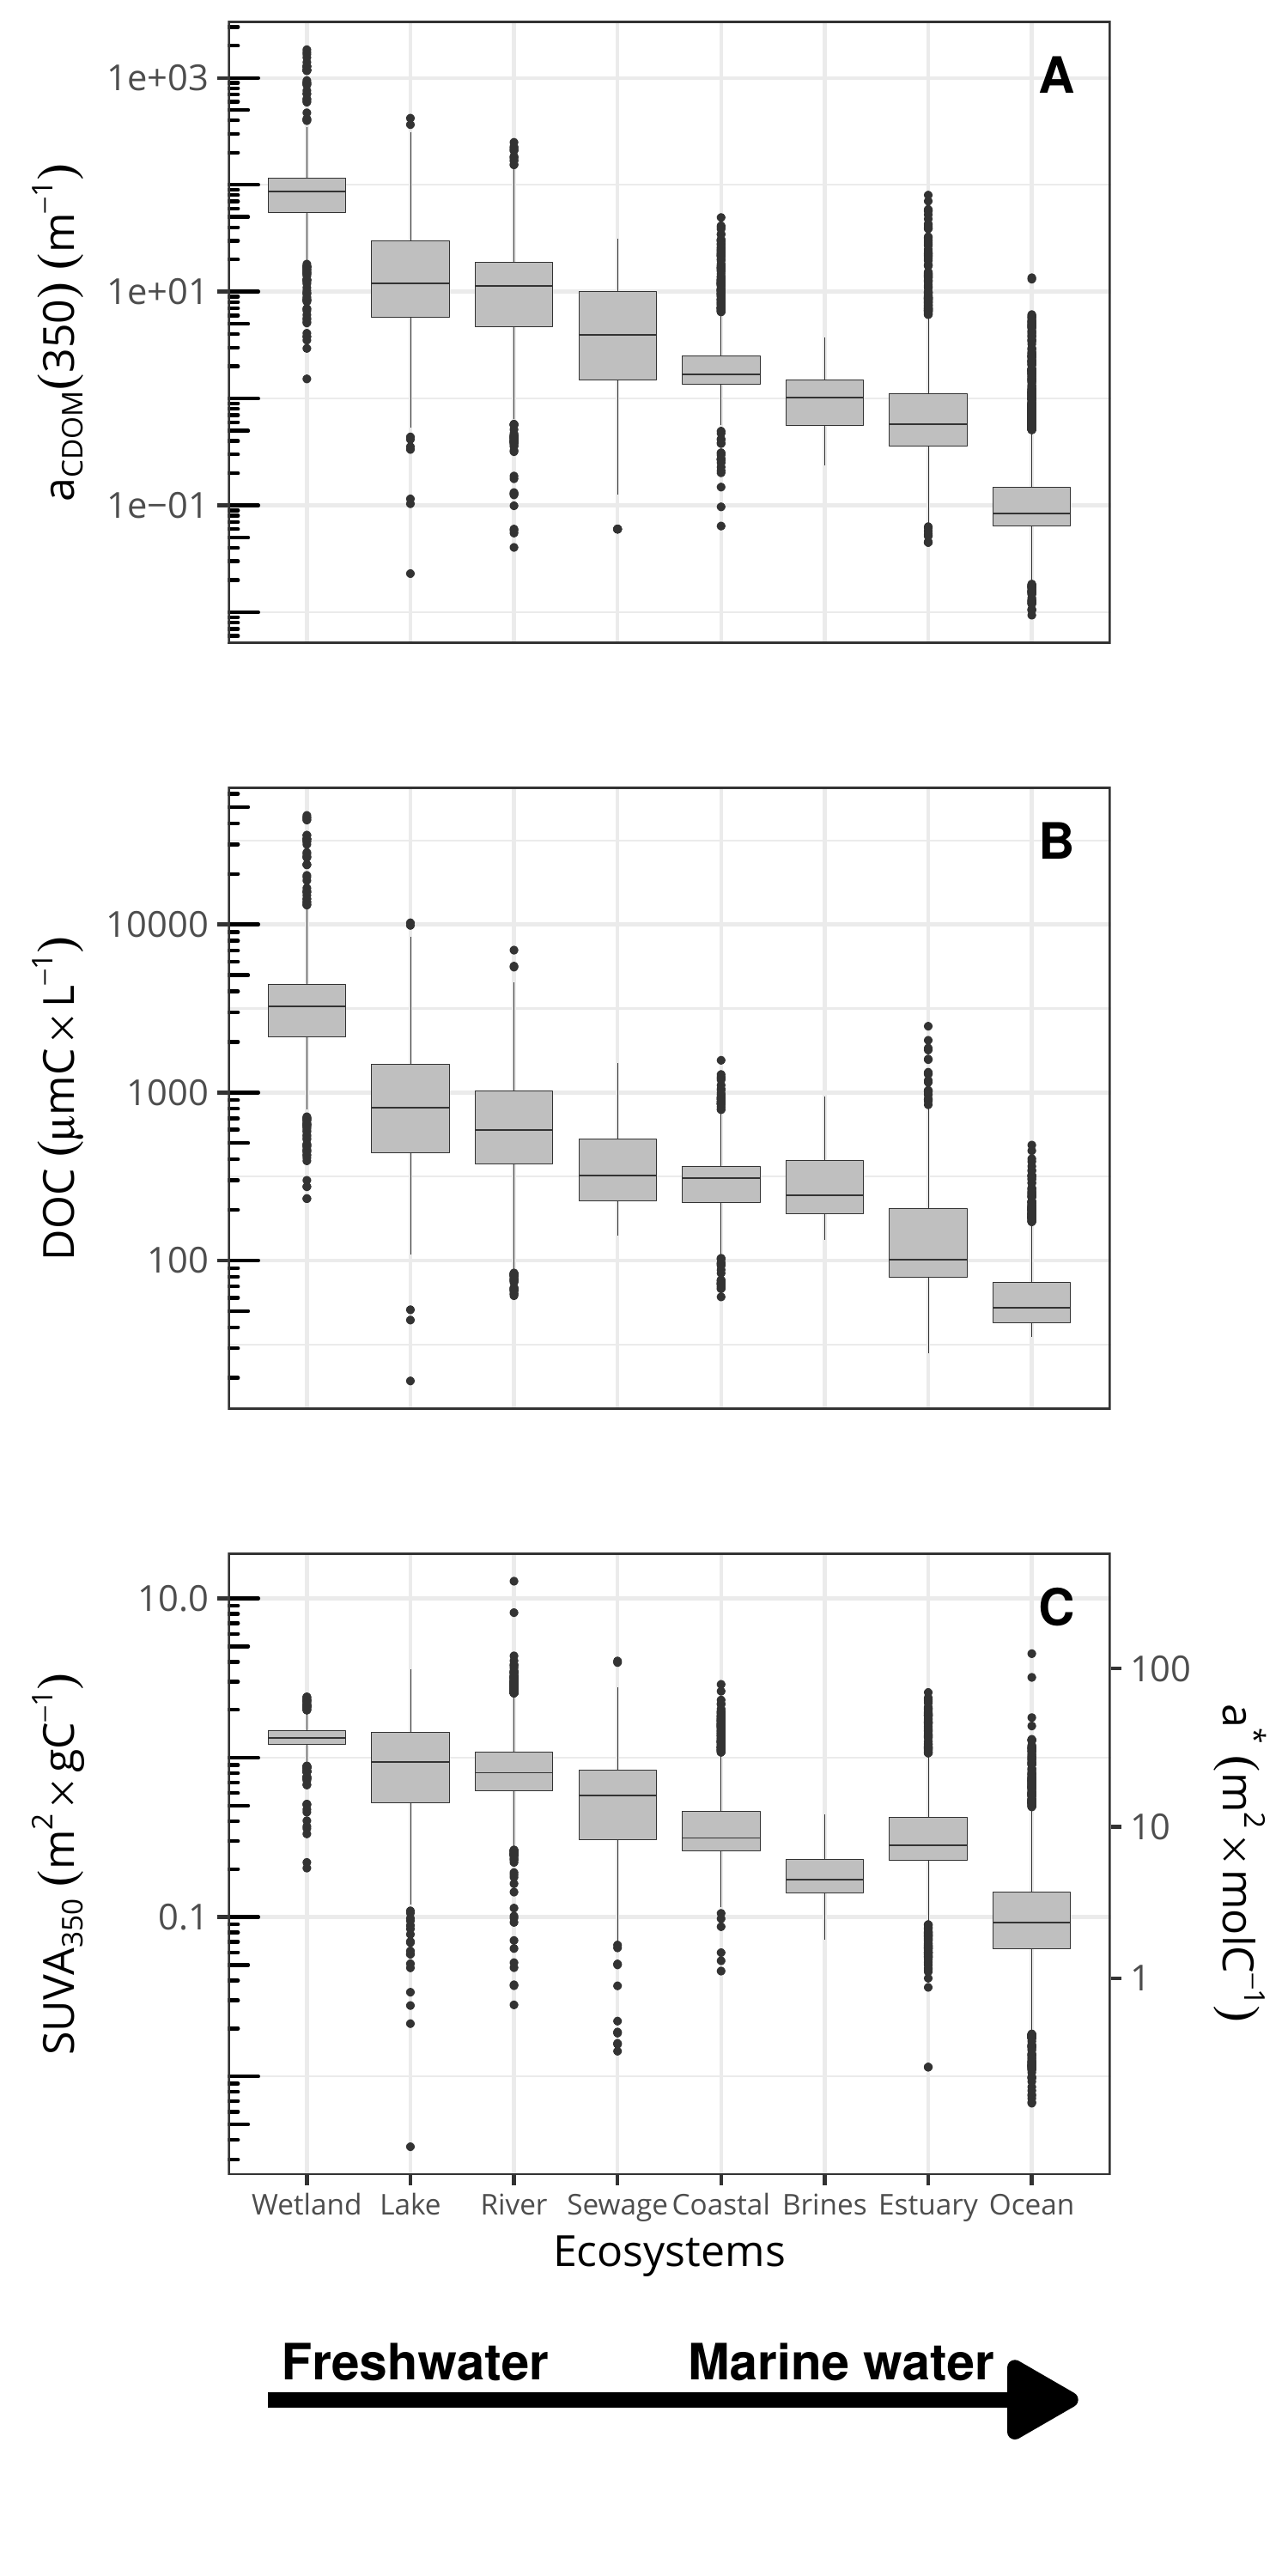
\includegraphics[scale = 1]{../../graphs/fig4}
	\caption{(\textbf{A}) Global relationship between absorption at 350 nm a\textsubscript{CDOM}(350) and dissolved organic carbon. The blue line is the fitted values of a linear model $y~=~log(x), R^2~=~0.93, p~<~0.00001, n~=~11562$. (\textbf{B}) Barplot showing the determination coefficient ($R^2$) of the linear relationships between a\textsubscript{CDOM}(350) and DOC by ecosystems. The dashed horizontal line represents the average of $R^2$.}
\end{figure}

\clearpage
\newpage

\begin{figure}[h]
	\centering
	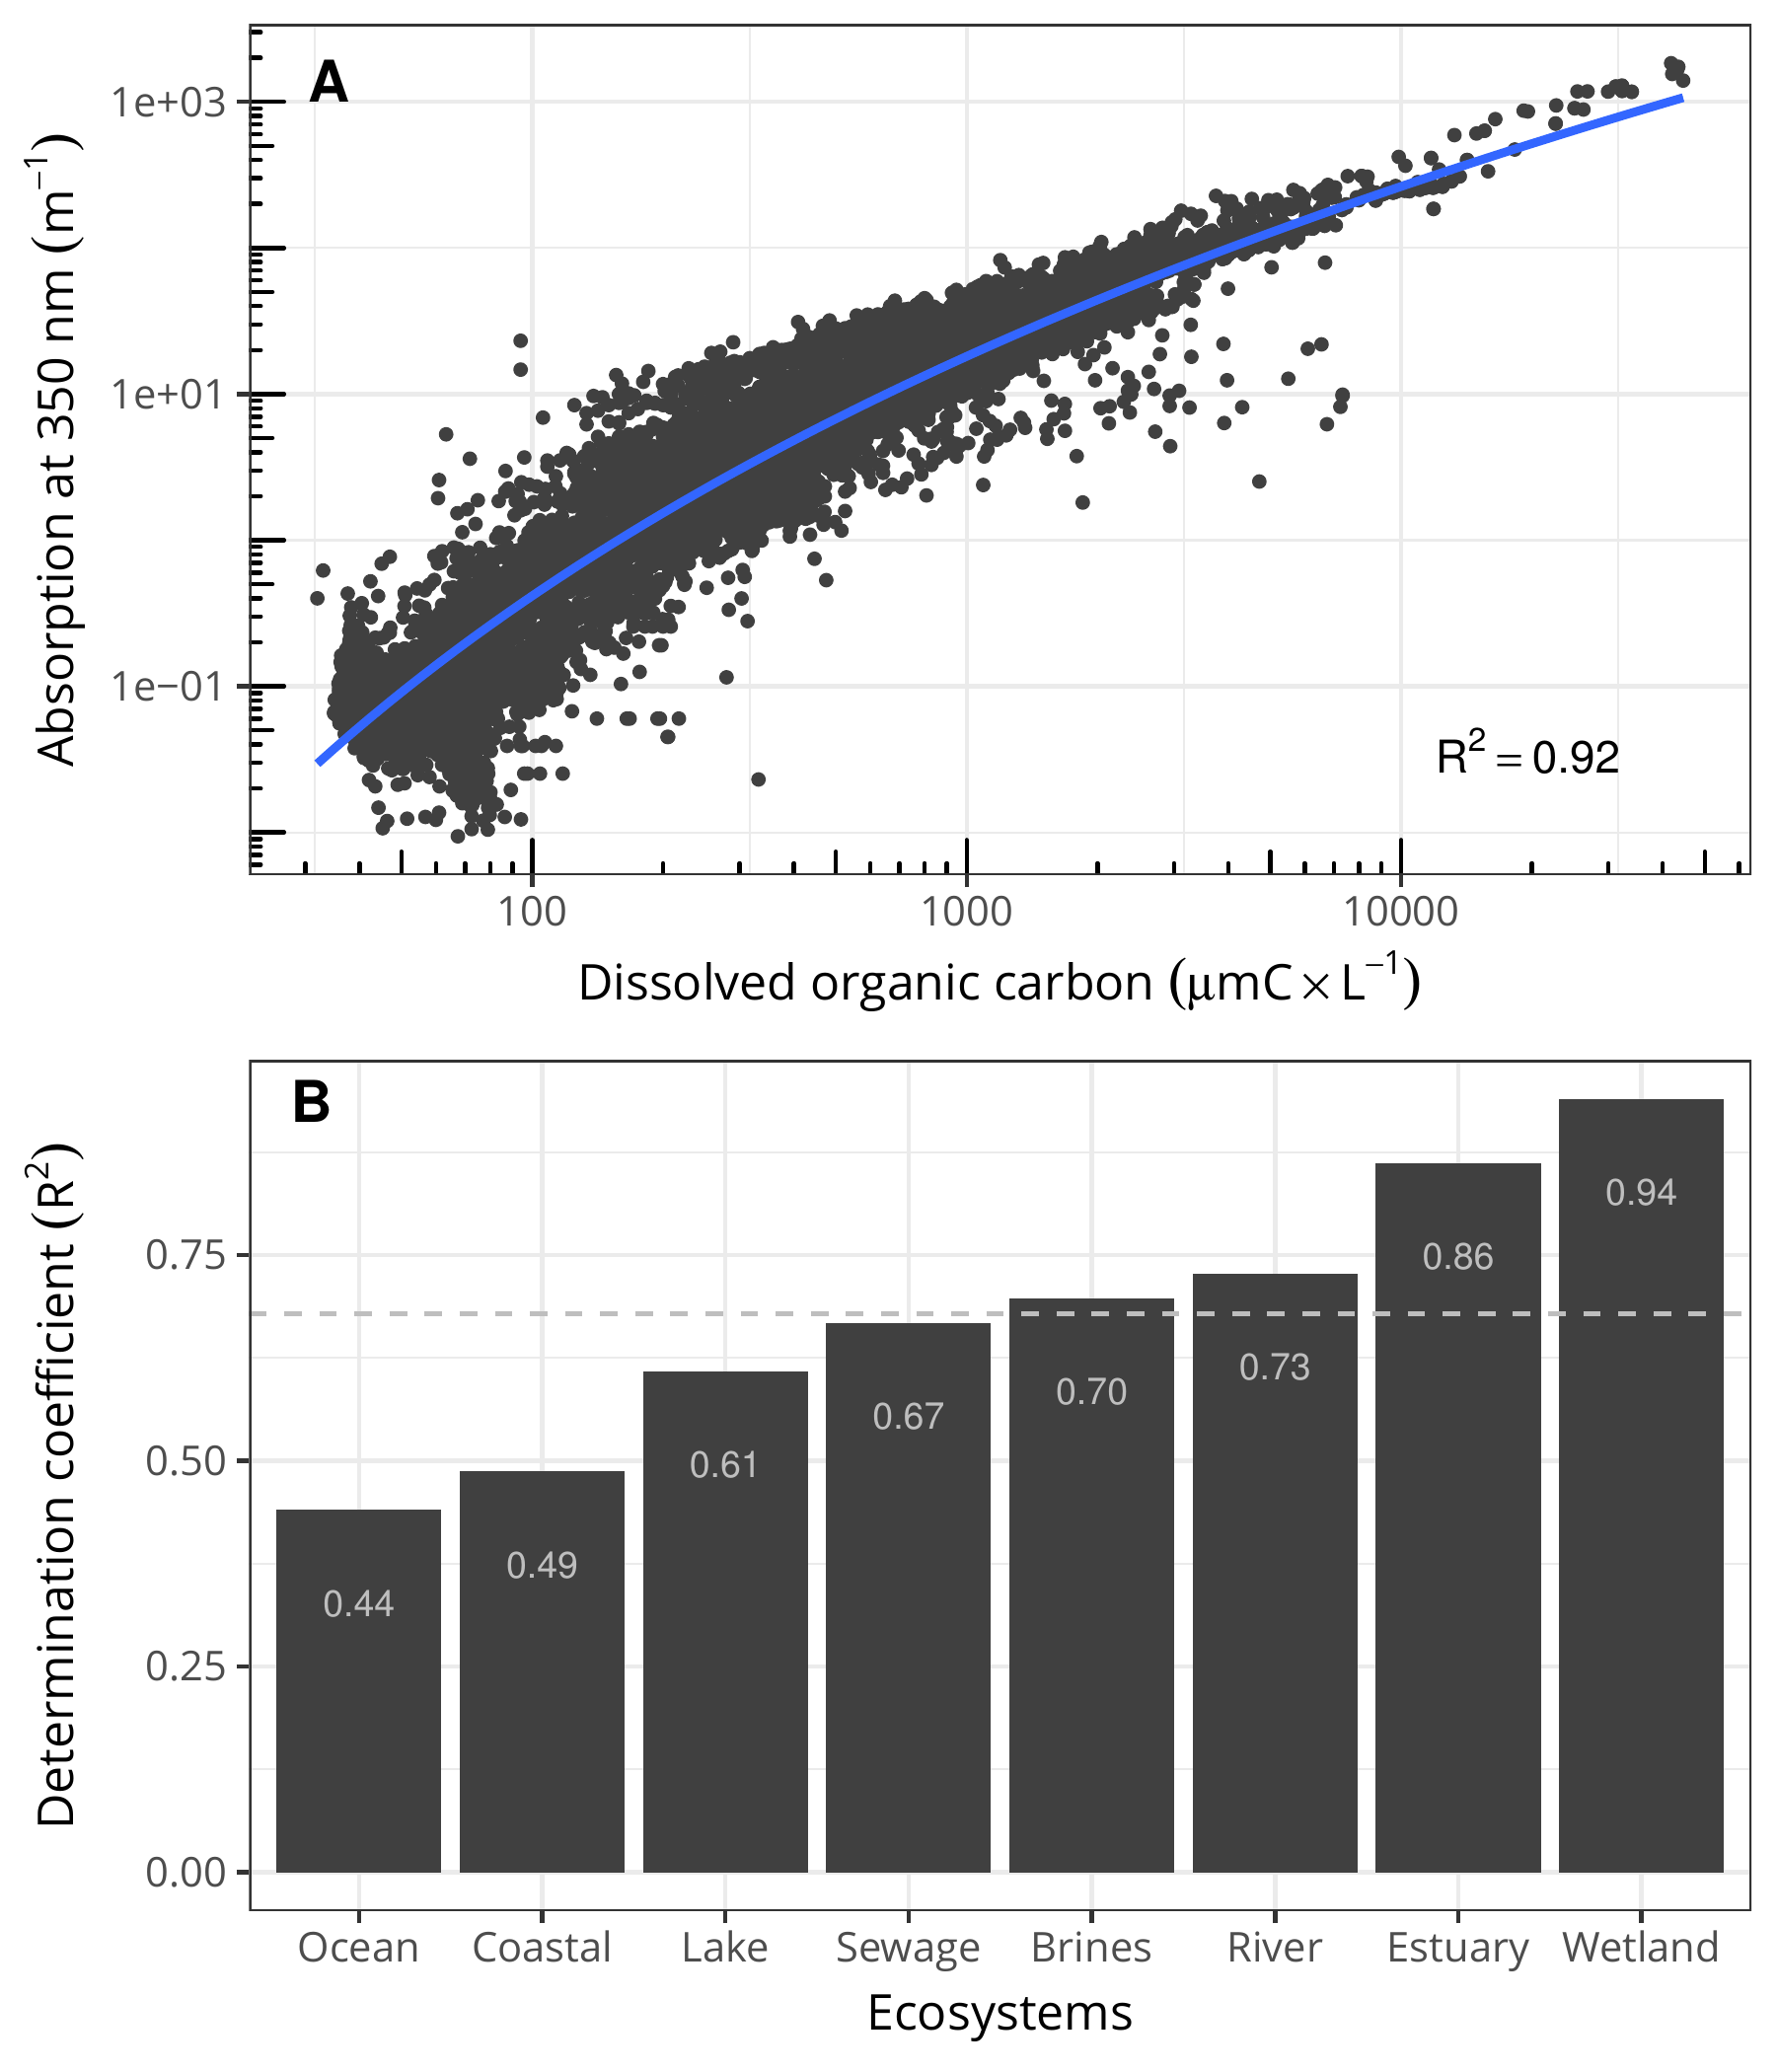
\includegraphics[scale = 1]{../../graphs/fig5}
	\caption{Segmentation analysis performed on the linear relationship between SUVA\textsubscript{254} and salinity ($R^2~=~0.74, p~<~0.00001, n~=~1841$). Dashed vertical lines represent the identified breakpoints at salinity 8.66 and 26.84.}
\end{figure}

\begin{figure}[h]
	\centering
	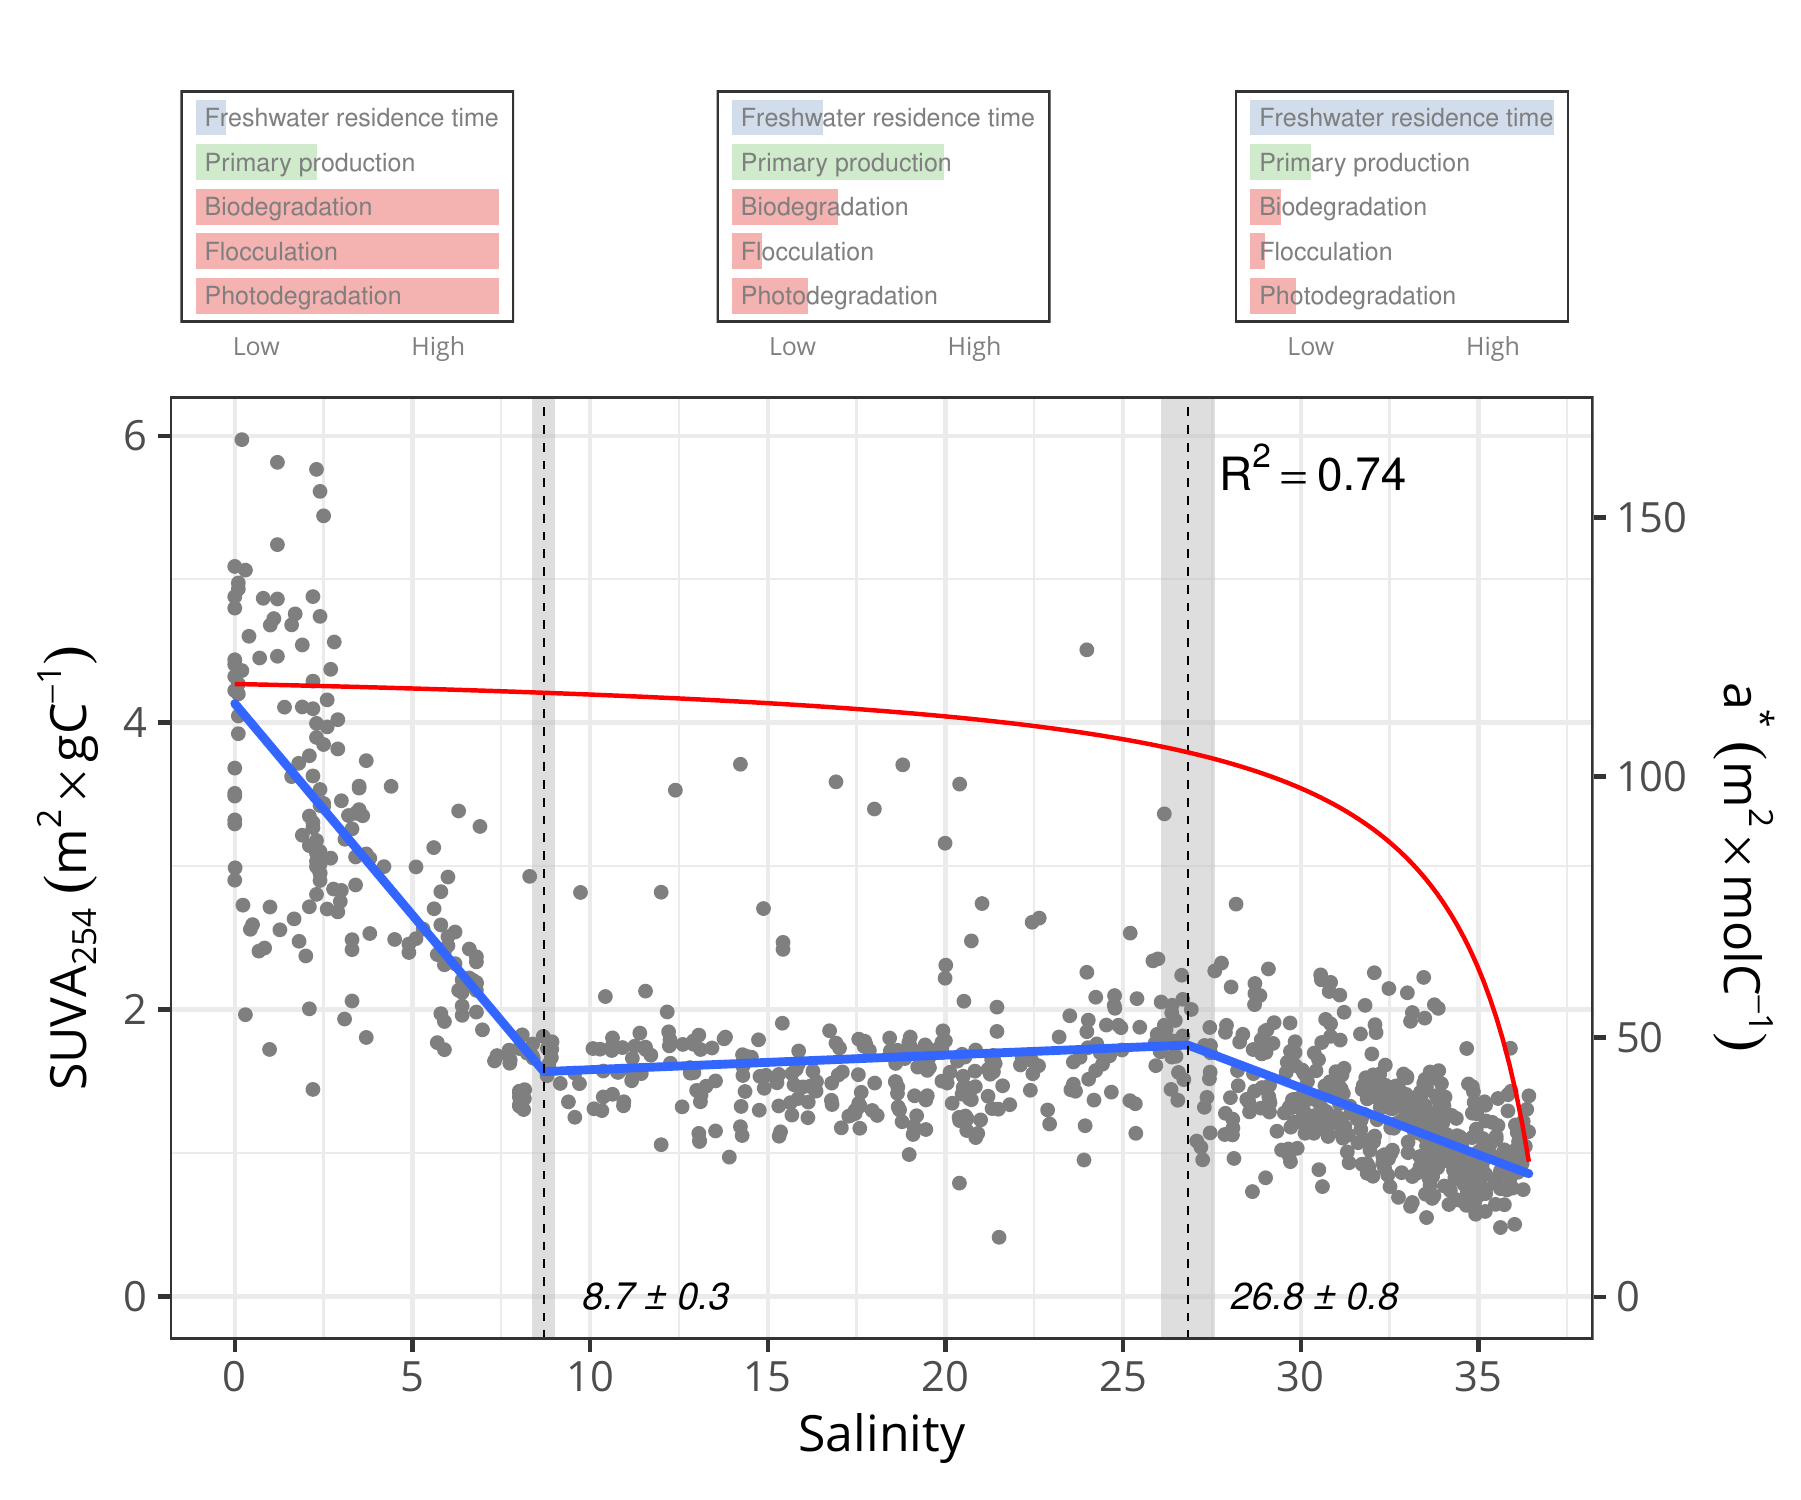
\includegraphics[scale = 1]{../../graphs/fig6}
	\caption{Principal component analysis showing the linear relationships between selected variables ($n = 1841$). The total variance explained by the first two principal components is 67.5\%.}
\end{figure}

\end{document}
